\documentclass[12pt,fleqn]{article}
\usepackage{xiiiemc}
\usepackage{natbib}
\usepackage[brazil,portuges]{babel}
\usepackage{fancyhdr}
\usepackage{color}
\usepackage{amsmath}
\usepackage{xcolor}
\usepackage{wallpaper} 
\usepackage{graphicx}
\usepackage{titlesec}   %% Define space between paragraph e section
\usepackage{float} 	%% Use to fix Figure or Table: ex: \begin{table}[H]
%%%%Don't edit this block. It reduces the spacing between the lines of the references
\let\OLDthebibliography\thebibliography
\renewcommand\thebibliography[1]{\OLDthebibliography{#1} \setlength{\parskip}{0pt}\setlength{\itemsep}{0pt plus 0.3ex}}

%%-----------------------------------------------EDIT-----------------------------------------------
\title{MODELAGEM COMPUTACIONAL - PROJETO 1:CIRCUITO RLC}

%%-----------------------------------------------EDIT----------------------------------------------
\author
    {\rm \begin{tabular}{l} 
    \textbf{Gabriel Calheias Alves}\\
    \textbf{Lizandra Moraes de Oliveira Jardim}\\
    \textbf{Moises Rangel Alves Filho}\\
    \textbf{Rayssa Montecchiari}\\
    \textbf{Vitor Saraiva de Lima}\\
  \end{tabular}}
%%----------------------------------------------------------------------------------------------
\fancypagestyle{firspagetstyle}
{   
    \lhead{}
	\fancyhead[C]{
	%%
\includegraphics[width=1\linewidth]{logo}\\%
		{\scriptsize \fontfamily{phv}\fontsize{18}{0}\fontseries{b}\selectfont \color[rgb]{0.45,0.45,0.45}
		Universidade do Estado do Rio de Janeiro\\
		Instituto Politécnico do Rio de Janeiro\\
		Nova Friburgo - RJ\\
	    }
	}
	\renewcommand{\headrulewidth}{0.1pt}
	\fancyfoot[C]{\footnotesize \parbox{10cm} {\centering  \fontsize{10}{0}\selectfont \it Rio de Janeiro, \today}} % \ttfamil
	\rhead{}
}
\fancypagestyle{pagetstyle}
{
    \lhead{}
	\fancyhead[L]{\footnotesize{\fontsize{10}{0}\selectfont \it MODELAGEM COMPUTACIONAL - PROJETO 1:CIRCUITO RLC}}
    \renewcommand{\headrulewidth}{0.1pt}
    \fancyfoot[C]{\footnotesize \parbox{10cm} {\centering  \fontsize{10}{0}\selectfont \it  Rio de Janeiro, \today}} % \ttfamil
    \rhead{}
}
\begin{document}
\pagestyle{pagetstyle}
\maketitle
\thispagestyle{firspagetstyle}

\begin{abstract}
Este documento mostra o passo a passo da modelagem física, matemática e computacional do projeto de um circuito RLC (Resistor(R), Indutor(L), Capacitor(C)) que tem por objetivo chegar ao valor da resistêcia para as condições L=5H, C=0.0001F, t=0.05s e carga igual a 1\% da carga inicial e do indutor para as condições  R=280 Ohms, C=0.0001F, t=0.05s e carga igual a 1\% da carga inicial.
\end{abstract}

\keywords{\em{RLC, Circuito, Resistor, Indutor, Capacitor }}

\pagestyle{fancy}

\section{INTRODUÇÃO}
Os engenheiros elétricos geralmente usam as leis de Kirchhoff para estudar o comportamento estacionário de circuitos elétricos. Outro problema importante envolve os circuitos que são transientes por natureza e em que ocorrem variações temporais súbitas. Tal situação ocorre depois que a chave na figura abaixo for fechada. Nesse caso, ocorrerá um período de ajuste após o fechamento da chave, até que um novo estado estacionário seja atingido. A duração desse período está intimamente ligada às propriedades de armazenamento do capacitor e do indutor. A presença de uma resistência no circuito irá dissipar o módulo das oscilações.\\

\textbf{Atividades de desenvolvimento:}\\
a)Determine uma expressão analítica para a variação da carga elétrica no circuito ao longo do tempo.\\
b)Determine o valor de R necessário para que o circuito dissipe a carga até atingir 1\% do seu valor original em t = 0,05 s, dado que L = 5 H e C = 0,0001F.\\
c)Determine o valor de L necessário para que o circuito dissipe a carga até atingir 1\% do seu valor original em t = 0,05 s, dado que R = 280 Ohms e C = 0,0001 F.

\section{MODELAGEM FíSICA}
O circuito a ser abortado no projeto é o mostrada na Fig. 1 e nele pode ser utilizada a segunda lei de kirchoff\cite{gussow2009eletricidade}. A segunda lei é a Lei de Kirchhoff para tensão, que afirma que a soma das tensões ao longo de um percurso fechado qualquer (malha) é igual à tensão total que está sendo fornecida a esse percurso , entao analisando o circuito separamos a malha da Fig.2 para a analise das tensões.
\begin{figure}[H] %h or !htbp
\vspace{-2pt}
\begin{center}
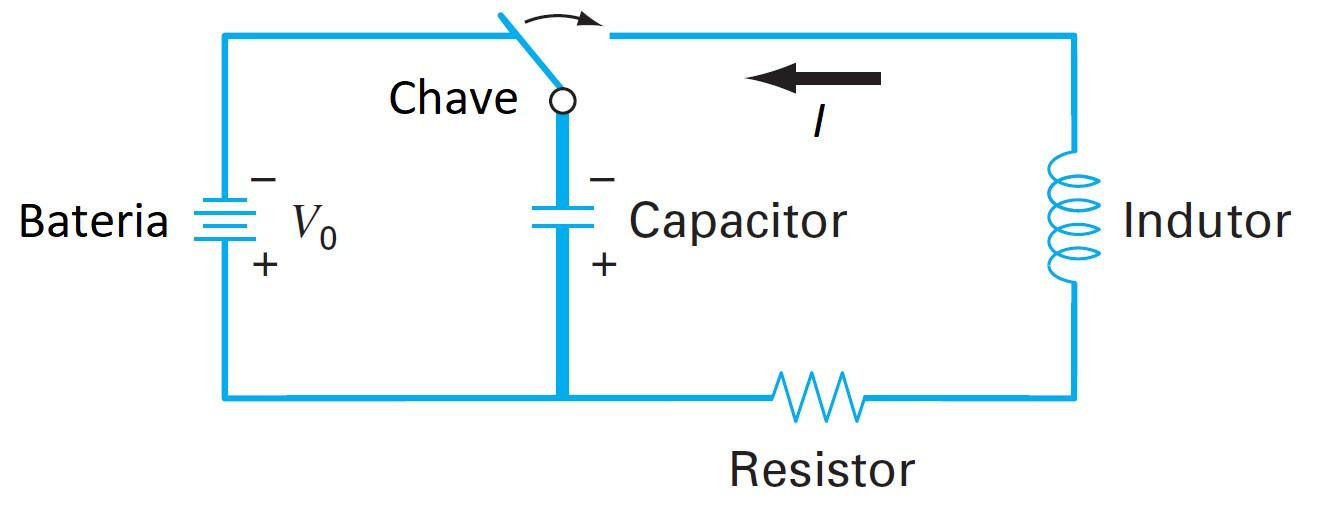
\includegraphics[height=5cm,width=12cm]{figura_1}%
\caption{Projeto 1:Circuito RLC}
\label{fig1}%
\end{center}
\end{figure}

\begin{figure}[H]%h or !htbp
\vspace{-2pt}
\begin{center}
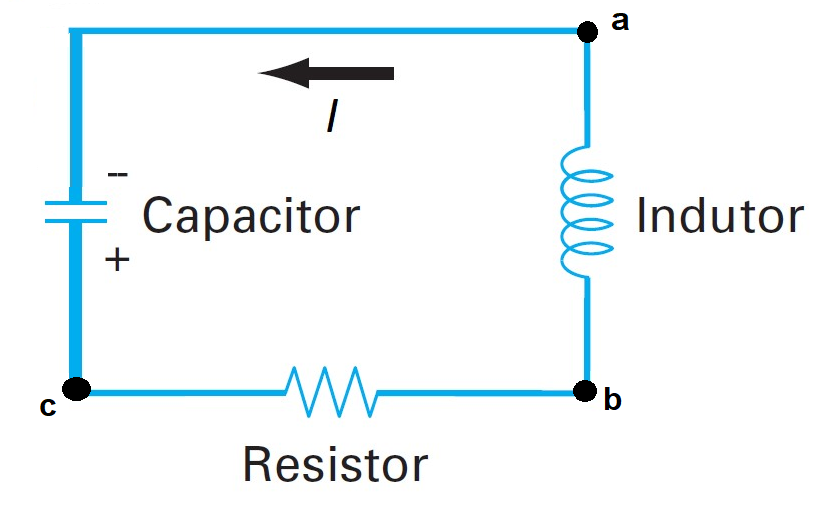
\includegraphics[height=5cm,width=8cm]{figura_2}%
\caption{Malha a ser analisada}
\label{fig2}%
\end{center}
\end{figure}

% \ \ \ \
\newpage %
\subsection{Segunda lei de Kirchoff}
 Após serem analisadas as tensões podemos ver que temos uma tensão no resistor, uma no indutor e outra no capacitor, isto é

\begin{equation}
V_{ab}+V_{bc}+V_{ca}=0
\label{eq}
\end{equation}

Podemos escrever a Eq. (1) em termos das correntes e cargas em cada um dos elementos do circuito, como a seguir.

\begin{subequations}
\label{eqn:total}
\begin{equation}
\label{eqn:parcial}
L\frac{\mathrm{d}i }{\mathrm{d} t}+Ri+\frac{q}{C}=0
\end{equation}

Sendo i = dq/dt, por definição de corrente elétrica, teremos:

\begin{equation}
L\frac{\mathrm{d^{2}q} }{\mathrm{d} t^{2}} +R\frac{\mathrm{d} q}{\mathrm{d} t}+\frac{q}{C}=0
\label{eqn:parcia1}
\end{equation}
\end{subequations}

Eq. (2b) é uma equação diferencial de segunda ordem, completa e homogênea. 

\section{MODELAGEM MATEMÁTICA}
A equação diferencial de segunda ordem\cite{boyce2017elementary} Eq. (2b) foi resolvida utilizando a equação característica abaixo:

\begin{equation}
L\alpha ^{2}+R\alpha +\frac{1}{C}=0\\ \equiv  \\\alpha ^{2}+\frac{R}{L}\alpha +\frac{1}{LC}=0
\label{eq}
\end{equation}

Após ser aplicado fórmula de Bhaskara e terminando a resolução da equação diferencial de segunda ordem temos:

\begin{equation}
q(t)=C_{1}e^{at}Cos(bt)+C_{2}e^{at}Sin(bt)\\ onde: \\a=-\frac{R}{2L}\\ b=\sqrt{\frac{1}{LC}-\left ( \frac{R}{2L} \right )^{2}}
\label{eq}
\end{equation}

Utilizando a Eq. (4) e aplicando as condições iniciais obtemos que 
\begin{subequations}
\label{eqt,total}
\begin{equation}
\label{eqt:parcial1}
C_{1}=q_{0}\\ C_{2}=\frac{-aq_{0}}{b}
\end{equation}

logo:

\begin{equation}
\label{eqn:parcia2}
q(t)=q_{0}e^{at}Cos(bt)-\frac{aq_{0}}{b}e^{at}Sin(bt)\\ com \\ q(t)=0.01q_{0}
\end{equation}
\end{subequations}

temos a nova função

\begin{equation}
f(x)=e^{at}Cos(bt)-\frac{a}{b}e^{at}Sin(bt)-0.01
\label{eq}
\end{equation}

onde a variável x pode ser o resistor (R) ou o indutor (L) se tornando uma f(R) ou f(L).

\section{MODELAGEM COMPUTACIONAL}
Utilizando a equação
\begin{equation}
f(x)=e^{-\frac{R}{2L}t}Cos\left ( \sqrt{\frac{1}{LC}-\left ( \frac{R}{2L} \right )^{2}} t\right )+\frac{\frac{R}{2L}}{\sqrt{\frac{1}{LC}-\left ( \frac{R}{2L} \right )^{2}}}e^{-\frac{R}{2L}t}Sin(\left ( \sqrt{\frac{1}{LC}-\left ( \frac{R}{2L} \right )^{2}} t\right ))-0.01
\label{eq}
\end{equation}

Podemos entao começar a resolver o problema aplicando um método númerico\cite{chapra2008metodos}.
\vspace{0.5cm}
Tendo em mente que a função dependento dos valores dados terá como x: R ou L, será utilizado o método da bisseção, que consiste em escolher um intervalo [a,b] que tenha a raiz da função nele e acharmos um valor aproximado da raiz. Para sabermos em qual intervalo há uma raiz será analisado o gráfico das funções e escolhido o melhor intervalo.
\vspace{0.5cm}
Após serem feitos os gráficos de f(R) e f(L) foi notado que o gráfico de f(L) não passava pelo eixo x logo, não seria possível achar o valor da raiz aproximada. Mas o gráfico de f(R) passava pelo eixo x então foi utilizado o método da bisseção na função f(R) e o valor obtido foi aproximado para o inteiro mais próximo e utilizado no valor de R da função f(L) chegando ao gráfico da Fig.6. 
\vspace{0.5cm}
Com os gráficos em mãos foi então utilizado o fluxograma da Fig. 3 para programar o método da bisseção na linguagem C++.

\begin{figure}[H] %h or !htbp
\vspace{-2pt}
\begin{center}
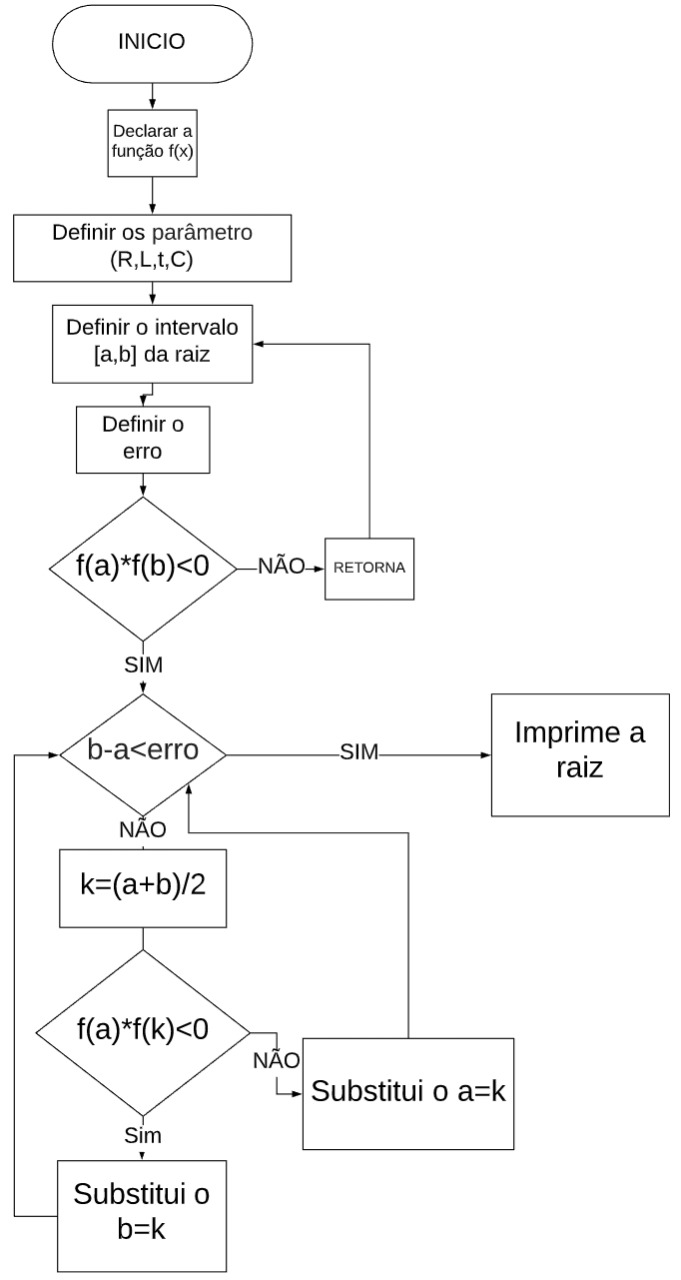
\includegraphics[height=18cm,width=12cm]{figura_3}%
\caption{Fluxograma Projeto}
\label{fig3}%
\end{center}
\end{figure}

\begin{figure}[H] %h or !htbp
\vspace{-2pt}
\begin{center}
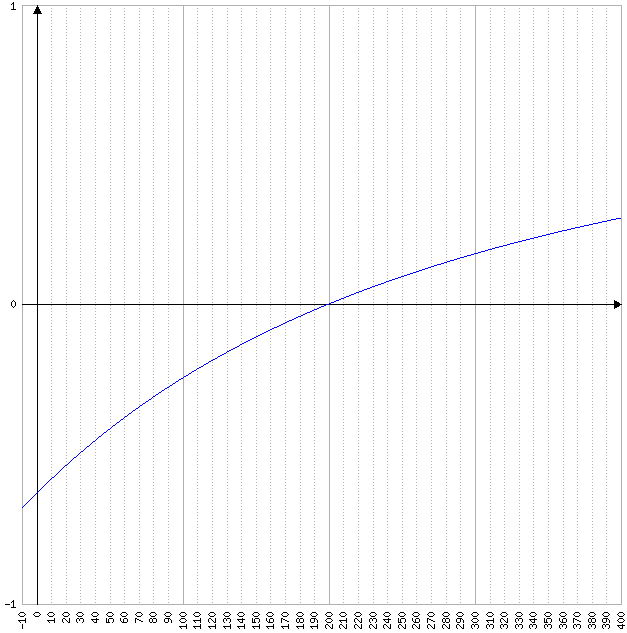
\includegraphics[height=10cm,width=10cm]{figura_4}%
\caption{Gráfico f(R)}
\label{fig4}%
\end{center}
\end{figure}

\begin{figure}[H] %h or !htbp
\vspace{-2pt}
\begin{center}
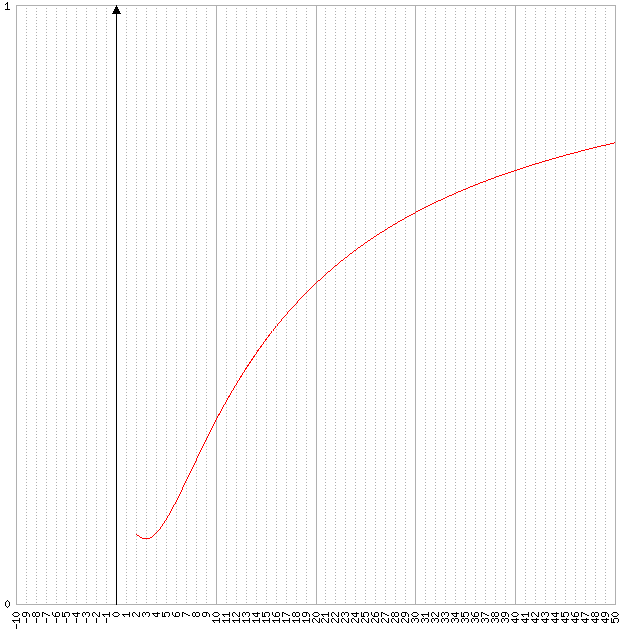
\includegraphics[height=10cm,width=10cm]{figura_5}%
\caption{Gráfico f(L) com R=280}
\label{fig5}%
\end{center}
\end{figure}

\begin{figure}[H] %h or !htbp
\vspace{-2pt}
\begin{center}
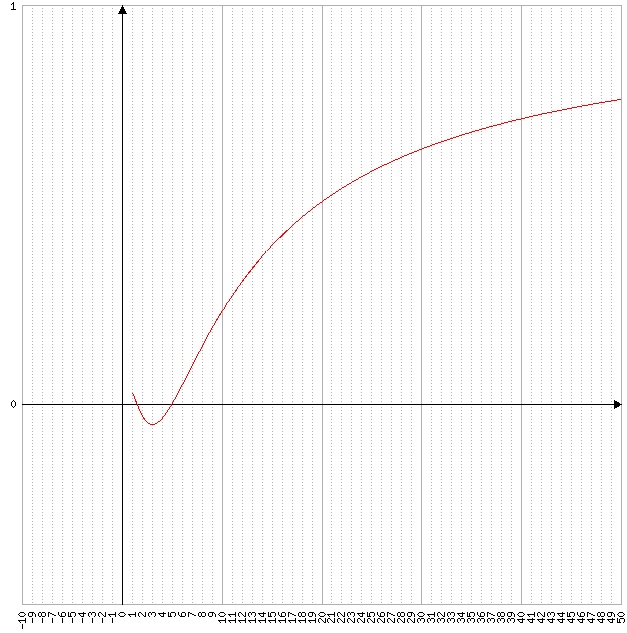
\includegraphics[height=10cm,width=10cm]{figura_6}%
\caption{Gráfico f(L) com R=200}
\label{fig6}%
\end{center}
\end{figure}

\section{RESULTADOS}
Após a aplicação do método da bisseção foram calculados os valores aproximados de R para o item b e de L para o item c, os valores aproximados calculados pelo programa foram:\\ \\
b) R= 197,93 Ohms, com o intervalo [0,400].\\
c) L = 1,50 H, com o intervalo [1,4] e L = 4,9 H, com o intervalo [2,6].

% ------------------------------------------------------------------------
\newpage
\bibliographystyle{plain}
\bibliography{modcomp}
\vspace*{-0.1cm}
% ------------------------------------------------------------------------


\begin{center}
\vspace{1cm}
  COMPUTER MODELING - PROJECT 1:RLC CIRCUIT
\end{center}

\def\abstractname{Abstract}%

\begin{abstract}
This document shows the step by step of the physical, mathematical and computational modeling of the design of an RLC (Resistor (R), Inductor (L), Capacitor (C)) circuit aiming to reach the resistance value for the conditions L = 5H, C = 0.0001F, t = 0.05s and charge equal to 1 \% of the initial charge and inductor value for conditions R = 280 Ohms, C = 0.0001F, t = 0.05s and charge equal to 1 \% of the initial charge.
\end{abstract}

\keywords{\em{RLC, Circuit, Resistor, Inductor, Capacitor}}

\end{document}
